%=============================================================================
% RELATED WORK
% Again, Simon Peyton Jones has a lovely description of how to write a paper on his website\endnote{\url{http://research.microsoft.com/en-us/um/people/simonpj/papers/giving-a-talk/giving-a-talk.htm}}. Personally, I put URLs in footnotes and \emph{bona fide} references in the bibliography. For instance, Turing \cite{turing37computable} and Knuth \cite{knuth68art} would not be out of place in list of references. How many references? Hard to say. Five is not enough, 50 is pushing it.

\documentclass[../mpaper.tex]{subfiles}
\begin{document}

Major research in Developer Experience has not been established yet as it is a new area becoming mainstream only recently. Like user experience, DX is subjective but it is made up of objective attributes. We aimed to understand developers, their preferences and their different experiences by asking questions that can provide context on their background and characteristics.

% \begin{figure}[h]
%     \centering
%     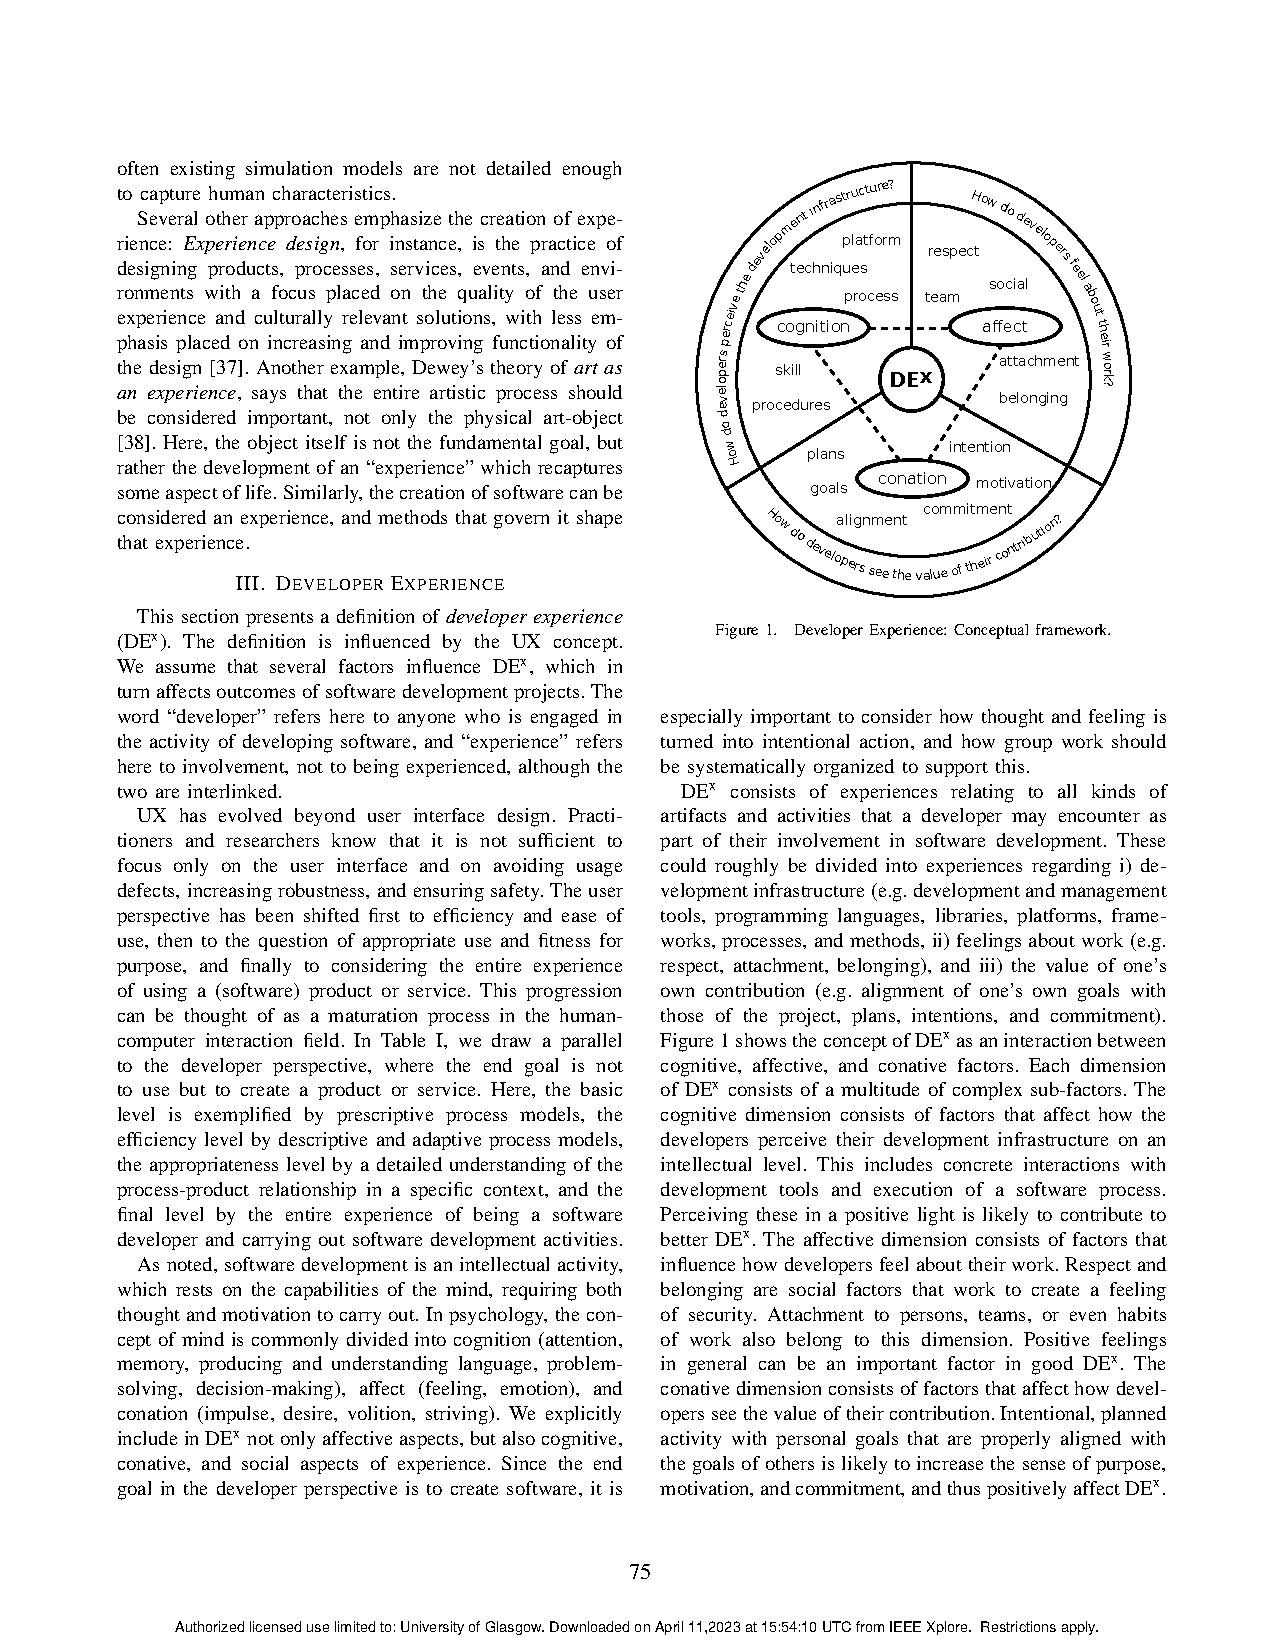
\includegraphics[trim={11.7cm 17.7cm 2.4cm 2.7cm},clip,width=0.4\textwidth]{Developer_experience_Concept_and_definition-3.pdf}
%     \caption{Conceptual framework for DX \cite{fagerholmDeveloperExperienceConcept2012}}
% \end{figure}

\subsubsection*{How do developers learn new tools?}

There are numerous tools available to develop software; this can be a new programming language or an external third-party library that provides some utility. A developer is different from a "non-developer" through knowledge of computing concepts and programming (writing code).

There are multiple ways to learn a new technology - there could be literature in form of a book or article, documentation hosted online, or a video tutorial. Producing these instructions (part of DevRel) involves human effort and requires the reader and writer to understand each other. \citet{kafer2017best} compare (passive) text-based tutorials with video-based tutorials to understand which is better in terms of efficiency and learning; they discovered negligible differences for either approach despite each having their own sets of advantages and disadvantages  \cite{alexanderUsabilityPrintOnline2013}. Text tutorials were completed faster \cite{mestreStudentPreferenceTutorial2012}, while video tutorials helped faster learning over the comparatively longer period \cite{lloydScreencastTutorialsEnhance2012,vandermeijComparisonPaperbasedVideo2014} and were preferred by the participants when given the choice. It is useful for developers to have both video demonstrations and written literature, but some tutorials should require practical exercises to be completed by the readers so that documentation does not serve to "spoon-feed" developers.

\citet{murphy-hillHowUsersDiscover2015} look into "social solutions" that allow developers to learn new tools; these include peer observations, tool encounter, and RSS feeds. Pair programming is a popular practice in software development and it also enables a great amount of tool discovery between developers \cite{cockburnCostsBenefitsPair2001} as it opens opportunity to observe other developer's tools and have discussions. Furthermore, \citet{begelNoviceSoftwareDevelopers2008} studies new recruits (novices) at Microsoft (a large organisation) to understand how they progress and transition to experts, finding that onboarding processes are tailored for this purpose and involve effective methods such as mentoring and pair-programming in the team. However, these rely on communication and the relationship between developers, and they may not share the same enthusiasm \cite{waiteStudentCultureVs2004,marzoloExtremeDevelopmentMeans2021}.

Most importantly, searching on the internet is an important, common step while learning new tools. \citet{baoTrackingAnalyzingCrossCutting2015} found that there are more than 20 queries made by developers every day -- a lot of it depends on the development phase, such as requirement analysis (where they search for explanations of terminologies, books and tutorials to understand business logic), the development phase (where they look for third-party libraries), or maintenance (looking for bugs that are commonly faced hopefully with a solution provided). Understanding queries also provides potential to understand developers' problems during the development process and possibly develop tools to help them. \citet{bajracharyaAnalyzingMiningCode2012,stoleeSolvingSearchSource2014} and \citet{sadowskiHowDevelopersSearch2015} investigate how developers make search queries for their tasks, revealing different dimensions of search along with corresponding frequencies in order to highlight the importance of developing domain-specific search engines, automated generation \& refinement of search queries, and knowledge sharing platforms; such solutions (like Stack Exchange) exist, but generating appropriate search queries (picking right keywords, adapting the traceback, etc) is an acquired development skill.

\subsubsection*{What do developers already know?}

Experienced (senior) developers are aware of many tools, but they can still discover new ones \cite{murphy-hillHowUsersDiscover2015}, especially with new solutions being created at a fast rate with software. For awareness of their activity \& practices, there are tools available to measure productivity, code health, test coverage and more; they work for projects most of the times, but they require high discipline and inference from the developers. There are also simple elements like autocomplete/IntelliSense and static analysers that provide feedback on code and developers must be able to diagnose and recover from the problems. \citet{lajiosSoftwareMetricsSuites2009} attempts to determine individual metric suites that fit into projects without correlating too highly with each other, for quality assessment \& defect prediction, using machine learning and applying Correlation-based Feature Selection (CFS); they learnt that Weighted Methods per Class (Chidamber \& Kemerer) and cyclomatic complexity (McCabe) were the most commonly suited metrics; these metrics may provide technical insight but they are not grounded to novice developers. \citet{blondeauSoftwareMetricsPredict2015} distinguishes metrics useful to predict the status of a project by conducting a literature review and evaluating a project at a major IT company; they learnt that metrics highly depend on the nature of each project as there are separate benchmarks \& understandings of customer requests.

\subsubsection*{What circumstances are developers in?}

Development is influenced by the structure of the process; it can involve working individually or in a team. Development experience \& productivity is perceived differently for teams \cite{ruvimovaExploratoryStudyProductivity2022}. Tasks may depend on others' availability and learning could accelerate through pair programming \cite{murphy-hillHowUsersDiscover2015}. \citet{cookeMeasuringTeamKnowledge2001} and \citet{lewisMeasuringTransactiveMemory2003} view teams as a primary mechanism for leveraging specialised knowledge; this is why a software team is staffed according to the distribution of knowledge of tools required for successful completion of a project \cite{walzSoftwareDesignTeam1993}; having only individuals with diverse knowledge is an insufficient condition to achieve quality performance in a software project \cite{farajCoordinatingExpertiseSoftware2000}. Lack of trust, difficulties in communication, and lack
of identification with project goals negatively impact the
success of projects \cite{smiteEmpiricalEvidenceGlobal2010}.

In a study by \citet{manteiEffectProgrammingTeam1981}, group structures (outlined as Chief Programmer Team and Egoless Programming Team) were compared and classified their performance for managing software projects based on task properties such as difficulty, size, duration, modularity, reliability, time and sociability; it was revealed that a hybrid model (Controlled Decentralised) team is highly effective. Similarly, \citet{sawyerSoftwareDevelopmentTeams2004} discusses the ways software developers organise information in archetypes of software development teams (Sequence, Group, and Network) discovering hybrid models to be good solutions. Other factors revealed by \citet{heTeamCognitionDevelopment2007} include frequency of meetings as having positive effects on team cognition, emails having no effect, and gender diversity strongly affecting cognition positively.

\citet{basili1979investigation} studied relationships between the size of a programming group and several software metrics; however, modern agile teams are considered to must have less than 8 members. In evaluating team structures, \citet{amritIdentifyingCoordinationProblems2012} sought coordination problems in teams using analysis tools and found clashes that were difficult to quantify accurately. \citet{lopez-fernandezDevOpsTeamStructures2022} studied teams in DevOps and classified them based on variables such as collaboration frequency, product ownership sharing, and autonomy, while \citet{nanJointEffectTeam2013} aimed to understand collaboration in open-source revealing that performance is directly proportional on size \& structural interdependency. Clearly, there are many variables to development processes depending on the structure developers work in.

\subsubsection*{What motivates developers to be productive?}

Research has been carried out to understand developer productivity and its influencing factors under different contexts; \citet{trendowiczChapterFactorsInfluencing2009} lists these based on over a hundred publications along with their experiences involving industrial projects, workshops and surveys on software productivity, eventually learning that productivity of software development processes would depend significantly on the capabilities of the developers along with the tools and methods that they use; \textit{the first step of quantifying productivity management is selecting the right metrics}.

More appropriate to large projects is to have experienced developers in their core team, hence \citet{gillProductivityImpactsSoftware1990} looked at how productivity could be related to experience and found that they were directly proportional, i.e. software engineers with more experience were more productive; but using resources to recruit such engineers revealed declining returns; instead, putting greater emphasis on the design phase of a project is associated with increased productivity.

\citet{lakhanpalUnderstandingFactorsInfluencing1993} found team cohesion to be the dominating factor in team performance, but this was using a one-time survey. \citet{canedoFactorsAffectingSoftware2019} revealed 37 factors to be pertinent to team productivity including collaboration \cite{clincySoftwareDevelopmentProductivity2003,stephanidisHCIInternational20152015}, team member availability \cite{deomeloInterpretativeCaseStudies2013,maxwellBenchmarkingSoftwareDevelopmentProductivity2000}, and ease of communication \cite{wagnerSystematicReviewProductivity2018,yilmazEffectiveSocialProductivity2016}, while there's also individual characteristics such as work experience \cite{deomeloInterpretativeCaseStudies2013} and skill/competence \cite{maxwellBenchmarkingSoftwareDevelopmentProductivity2000,oliveiraSoftwareProjectManagers2016}. \citet{ruvimovaExploratoryStudyProductivity2022} carried out a study in a practical environment with 25 individuals across five software teams reporting their perceived productivity for themselves and their team over interviews and surveys, and the most important finding from their study was realising that teams in modern organisations are highly fluid varying in size, members, structure and projects causing different aspects and dependencies to productivity. Similar to the previous question's study in this section, we realise that there are more complexities and steps in a developer's productivity.

\subsubsection*{How do developers manage their workload?}

With respect to developers' personal lives and emotions, prioritising tasks is a crucial part of the process. Developers may switch between tasks based on their mental context or prioritise based on urgency. There have been established methods, such as Planning Poker, and software, such as Jira, to detail \& organise tasks. \citet{alhamedEvaluationContextAwareLanguage2022} describe limitations in effort estimation using planning poker, and use NLP models to predict estimates. Often, tasks can be seen as writing code (bugfix or new feature), tests or documentation. Developers tend to do these in a cyclic sequence -- write code, write tests for it and then document the change; however switching between these may be difficult creating fatigue and developers tend to prefer working on one area, like writing code and no tests and documentation causing code-tasks to be prioritised. Moreover, \citet{storerBehaveNicelyAutomatic2019} point out frustrations in maintaining test cases in Behaviour Driven Development (BDD), and use NLP algorithms to create tests so that there is only one area of code to maintain for developers \cite{binamunguMaintainingBehaviourDriven2018}. Along with that, information may not be central to Source Control Management (SCM) requiring more switching, so \citet{edwardsSciitEmbeddingIssue2021} study and embed issues into the SCM to help reduce friction and the additional maintenance required by a developer. These have paved the way to develop solutions central to the SCM that help developers manage their tasks.

\subsubsection*{Summary -- what did we find?}

The field of software development has been extensively researched, and the literature has provided valuable insights into the various complexities involved in the process. One of the main conclusions drawn from this research is that software development is not a linear path; it is a highly iterative and constantly evolving process, with multiple influencing factors like team cohesion, learning curves, requirement comprehension, and communication. These factors can impact the speed and efficiency of the development process, therefore the quality of the final product.

However, the minor gaps we found in the literature come from the limited scope focusing only on a narrow range of contexts and failing to consider the wider ecosystem in which development processes take place. Developer Experience \& Productivity has not been looked in both subjective and objective perspectives directly relating to developers' actions; there has also been relatively little focus on reducing friction in development, through tools or automation, that could significantly impact the dynamics of the process.

Our designed solution aims to solve this by providing a holistic view of developers' work-time, taking into account of their activity, efforts and the different contexts in the subjective developer experience, to provide more accurate and realistic measures for their productivity. This would enable us to gain a deeper understanding of the factors that influence software development and identify new ways to improve outcomes for both developers and organisations to ensure projects are completed on time and within budget.

\end{document}
